\graphicspath{ {./content/method/figures/} }
\onecolumn
\begin{landscape}

\begin{figure*}[Ht]
  \centering
  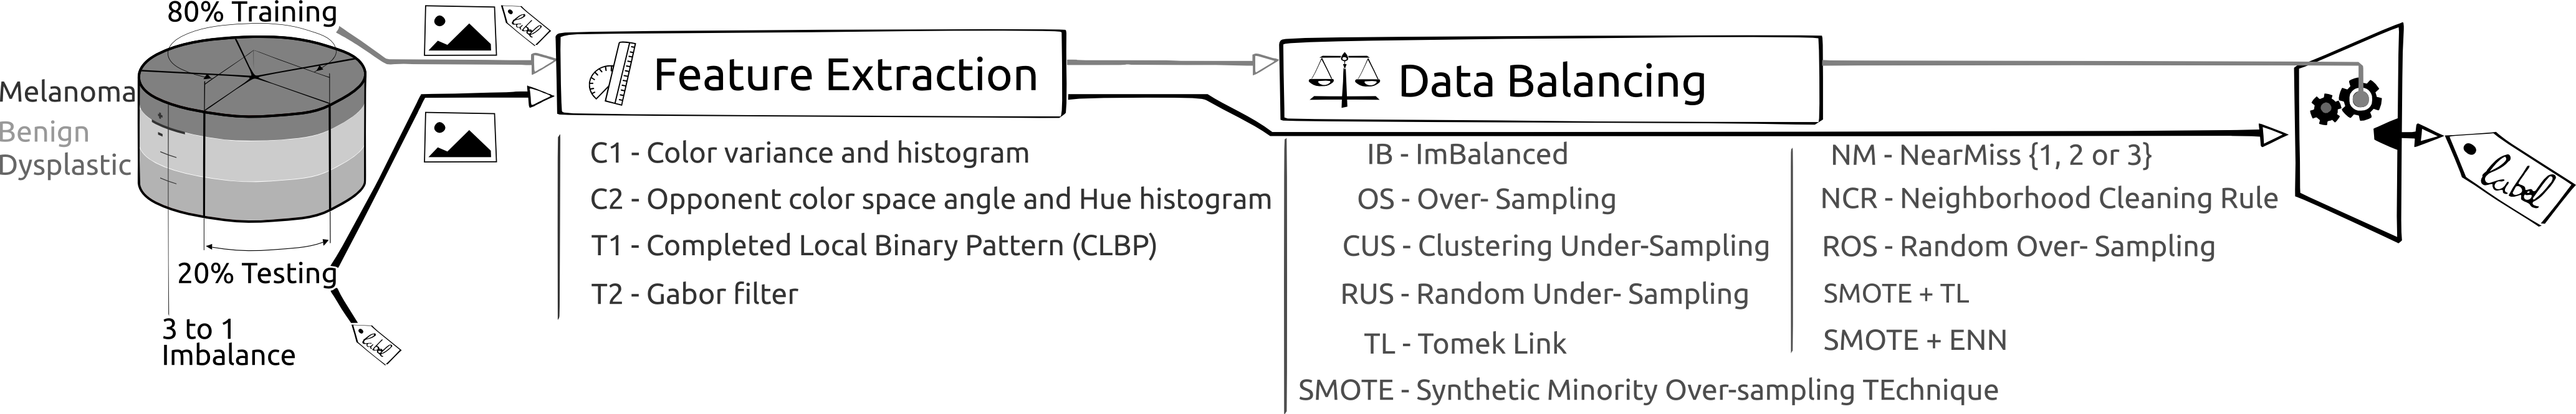
\includegraphics[width=1.4\textwidth]{method.png}
  \caption{Framework outline}
	\label{fig:schema}
\end{figure*}

\begin{table*}
\caption{The obtained results with different balancing techniques for color and texture features using a \acs*{rf} classifier. The first and second highest results for each feature set are highlighted in dark and lighter gray colors, respectively.}
\centering
\resizebox{1.42\textwidth}{!}{
\begin{tabular}{l cccccc		cccccc		cccccc}
\toprule
Features &  \multicolumn{6}{l}{Color}& \multicolumn{6}{l}{Texture} & \multicolumn{6}{l}{Combined}\\
  \cmidrule(r){2-7}  \cmidrule(r){8-13}  \cmidrule(r){14-19}  
		   & \multicolumn{2}{c}{$C_{1}$}& \multicolumn{2}{c}{$C_{2}$}& \multicolumn{2}{c}{$C_{1,2}$}& \multicolumn{2}{c}{$T_{1}$} &  \multicolumn{2}{c}{$T_{2}$} & \multicolumn{2}{c}{$T_{1,2}$}& \multicolumn{2}{c}{$T_{1},C_{1,2}$}& \multicolumn{2}{c}{$T_{2},C_{1,2}$}& \multicolumn{2}{c}{$T_{1,2},C_{1,2}$}\\ 
  \cmidrule(r){2-3}  \cmidrule(r){4-5} \cmidrule(r){6-7} \cmidrule(r){8-9} \cmidrule(r){10-11} \cmidrule(r){12-13} \cmidrule(r){14-15} \cmidrule(r){16-17} \cmidrule(r){18-19} 
  Balancing techniques & \makebox[0.5cm][l]{\acs*{se}}& \makebox[0.5cm][l]{\acs*{sp}} & \makebox[0.5cm][l]{\acs*{se}} & \makebox[0.5cm][l]{\acs*{sp}} & \makebox[0.5cm][l]{\acs*{se}} &\makebox[0.5cm][l]{\acs*{sp}} &\makebox[0.5cm][l]{\acs*{se}} &\makebox[0.5cm][l]{\acs*{sp}} &\makebox[0.5cm][l]{\acs*{se}} & \makebox[0.5cm][l]{\acs*{sp}} &\makebox[0.5cm][l]{\acs*{se}} &\makebox[0.5cm][l]{\acs*{sp}} & \makebox[0.5cm][l]{\acs*{se}} &\makebox[0.5cm][l]{\acs*{sp}} &\makebox[0.5cm][l]{\acs*{se}} &\makebox[0.5cm][l]{\acs*{sp}}& \makebox[0.5cm][l]{\acs*{se}} &\makebox[0.5cm][l]{\acs*{sp}}  \\ \midrule
\multicolumn{1}{c}{IB} & 52.50 & 89.58 & 75.00 & 88.75 & 71.25& 87.50& 38.75 & 91.67 & 60.00 & 96.25 & 66.25 & 93.75 &73.75 & 89.58&71.25 & 89.58 & 71.25& 92.50\\
\midrule \midrule
\multicolumn{1}{c}{\acs*{os}} &\cellcolor[gray]{0.6}93.75 &\cellcolor[gray]{0.6}66.67 &80.00 & 86.25& 82.50 & 87.08  & 43.75 &83.75 &\cellcolor[gray]{0.6}72.50&\cellcolor[gray]{0.6}90.00 & 70.00& 91.67  &77.50 & 87.08 &81.25 &88.33 &78.75 &88.33  \\
\midrule \midrule
\multicolumn{1}{c}{\acs*{ros}} &55.00 & 80.83& 80.00 & 84.17& 72.50 &85.42 &42.50 & 82.08 &60.00 & 89.17 &66.25 &87.92&75.00&85.42&73.75&86.25&73.75 &85.83\\
\multicolumn{1}{c}{\acs*{smote}} & 60.00 & 82.50 & 78.75 & 84.58 & 75.00 & 70.00 & 56.25 & 74.17 & 61.25 & 87.50 & 84.17 &87.08 & 78.75& 85.00 &73.75 & 84.58 &73.75&85.00 \\ 
\hdashline \noalign{\vskip 3pt}
\multicolumn{1}{c}{\acs*{rus}} & 72.50 & 72.92 & 86.25 & 80.00 & 78.75 &80.00 & 67.50 & 53.33 &76.25 &76.25  & 85.00 &78.75 &91.25 &75.00 & 85.00 & 78.75 &\cellcolor[gray]{0.6}92.50 &\cellcolor[gray]{0.6}78.33\\
\multicolumn{1}{c}{\acs*{tl}} & 51.25 & 86.25 & 76.25 & 87.92&67.50 & 88.33  & 37.50 & 87.92 & 65.00 &90.42 & 68.75 & 91.67 & 73.75 & 88.75 &63.75 & 90.00 & 72.50 & 91.25\\
\multicolumn{1}{c}{\acs*{cus}} & 81.25 & 67.92 & 80.00 & 84.58& 86.25 & 80.42 & 56.25 & 65.83 & 70.00 & 77.50 & 85.00 & 77.08 & 83.75 & 81.25 & 80.00 & 84.17 & 83.75 & 82.92\\
\multicolumn{1}{c}{\acs*{nm1}} & 67.50 & 72.08 & 86.25 & 79.17& 85.00 & 82.50 & 72.50 & 43.75 & 80.00 & 62.50 & 87.50 & 66.67 & 85.00 & 82.08 & 86.25 &80.42 & 87.50 & 80.83\\
\multicolumn{1}{c}{\acs*{nm2}} & 70.00 & 72.92 & 86.25 & 81.25 & 85.00 & 82.92 & 76.25 & 48.75 & 86.25 & 40.83 & 86.25 & 51.25& \cellcolor[gray]{0.6}87.50 & \cellcolor[gray]{0.6}82.08 &\cellcolor[gray]{0.6}92.50 &\cellcolor[gray]{0.6}77.50& 91.25 &81.67\\
\multicolumn{1}{c}{\acs*{nm3}} & 82.50 & 75.00 & 87.50 & 80.83 & 85.00 & 80.42 &73.75 & 55.83 & 72.50 & 82.50 & 82.50 & 80.42 & 83.75 & 81.25 & 85.00 & 80.00 & 86.25 & 80.42\\
\multicolumn{1}{c}{\acs*{ncr}} & 66.25 & 76.67 & \cellcolor[gray]{0.6} 87.50 &\cellcolor[gray]{0.6}81.25 & 85.00 & 82.08 & 67.50 & 67.92 & 75.00 & 85.83 & \cellcolor[gray]{0.6}82.50 & \cellcolor[gray]{0.6}83.33 &  86.25 &  81.67 & 82.50  & 85.00 & 83.75  & 85.42\\
\hdashline \noalign{\vskip 3pt}
\multicolumn{1}{c}{\acs*{smote} + \acs*{enn}} & 76.25 & 73.33 & 85.00 & 81.25 & 85.00 & 82.08 &\cellcolor[gray]{0.6} 81.25 &\cellcolor[gray]{0.6} 56.25 & 76.25 & 82.08 & 80.00 & 79.58 & 86.25 & 81.25 & 83.75 & 82.50 & 78.75 & 82.92\\
\multicolumn{1}{c}{\acs*{smote} + \acs*{tl}} & 75.00 & 73.75 & 83.75 & 82.50 & \cellcolor[gray]{0.6}87.50 &\cellcolor[gray]{0.6}80.83 & 72.50 & 59.17 & 77.50 & 82.08 & 78.75 & 78.75 & 85.00 & 82.08 & 77.50 & 82.92 & 88.75 & 82.50\\
\bottomrule
\end{tabular}
}
\label{tab:tab1}
\end{table*}

\normalsize \vfill
\end{landscape}
\twocolumn
